%------------------------------------------------------------
%
\documentclass[landscape, notitlepage]{article}%
%Options -- Point size:  10pt (default), 11pt, 12pt
%        -- Paper size:  letterpaper (default), a4paper, a5paper, b5paper
%                        legalpaper, executivepaper
%        -- Orientation  (portrait is the default)
%                        landscape
%        -- Print size:  oneside (default), twoside
%        -- Quality      final(default), draft
%        -- Title page   notitlepage, titlepage(default)
%        -- Columns      onecolumn(default), twocolumn
%        -- Equation numbering (equation numbers on the right is the default)
%                        leqno
%        -- Displayed equations (centered is the default)
%                        fleqn (equations start at the same distance from the right side)
%        -- Open bibliography style (closed is the default)
%                        openbib
% For instance the command
%           \documentclass[a4paper,12pt,leqno]{article}
% ensures that the paper size is a4, the fonts are typeset at the size 12p
% and the equation numbers are on the left side
%
\usepackage{graphicx,showexpl,listings}
\usepackage{tikz}
\usetikzlibrary{shapes.symbols, 
		shapes.geometric,
		arrows,
		decorations.pathmorphing,
		positioning,
		backgrounds,
		fit}
%-------------------------------------------

\begin{document}
\pagenumbering{gobble}
\topmargin=-10pt
\footskip=0pt
\center\small{Component Interaction: \large{SQW Data System}}

\begin{tikzpicture}[place/.style={
					circle,
					draw=blue!50,fill=blue!20,thick,
					inner sep=0pt,minimum size=6mm},
			component/.style={
					rectangle,
					draw=black!50,fill=blue!20,thick,
					minimum width=3cm,
					inner sep=10pt},
			innercomponent/.style={component, 
						       dotted, 
						       minimum width=0, inner sep=5pt},
			outsys/.style={component, fill=black!20},
			unused/.style={component,fill=black!10,dotted},
			inlay/.style={
					rectangle,
					draw=black!60,thick,dotted,
					minimum size=15mm,
					inner sep=2pt},
			%every label/.style=red,
			tinyfont/.style={font=\it\tiny},
			smallfont/.style={font=\it\small},
			elab text/.style={tinyfont,align=center},
		      elab/.style={above,elab text},
			elabb/.style={below,tinyfont,elab text},
			elabs/.style={above,sloped,elab text},
			elabbs/.style={below,sloped,elab text},
			end point/.style={circle,fill=red!30,draw=black!30,thick,
						 inner sep=1pt,
						 minimum size=5mm},
			database/.style={cylinder,draw,align=center,
						 fill=green!20,
						 aspect=.10,
						 minimum size=1cm,
						 minimum height=1cm+20pt,
						 inner sep=2pt,
						 shape border rotate=90},
			multipledb/.style={database,smallfont},
			returning/.style={dotted,bend angle=10,bend left},
			this is/.style=dotted,
			ital/.style={font=\itshape},
			subsys/.style={fill=red!10,ital,inner sep=5pt},
			bend angle=20,
			pre/.style={<-,shorten <=1pt,>=stealth',semithick},
			post/.style={->,shorten >=1pt,>=stealth',semithick}]
%% -------------- GRID ----------------------------------------- %%
	\path[help lines, blue!20, draw] grid (12,12);

%% --------------- SPEED LAYER ------------------------------ %%
\node [component, xshift=20pt, yshift=-5pt] (streamproc) at (2, 11) {Stream Processor};

\node [above=of streamproc,xshift=20pt,yshift=-1cm,ital] (speedtitle) {Speed Layer};
\node [database,right=of streamproc] (speeddb) {Recent Data\\R/W};

%% --------------- GATEWAY ------------------------------ %%
\node [component, below=of streamproc, xshift=0pt,yshift=-10pt] (ghreads) {Read Handler};

\node [below=of ghreads,xshift=-5pt,yshift=20pt,ital] (gtitle) {Gateway};

\node [component, below=of ghreads,xshift=0pt, yshift=0cm] (ghwrites) {Write Handler};

\node [innercomponent,
	below=of ghwrites,xshift=27pt,yshift=15pt]	(gser) {Serializer};

%% ---------------- CLIENT FIGURES ------------------------ %%
\node [left=of ghreads,xshift=10pt, yshift=1cm-10pt] (read) 
		{ 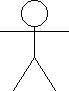
\includegraphics[width=0.4cm]{../img/stick.png}};

\node [ left=of ghwrites,xshift=10pt, yshift=-20pt] (write) 
		{ 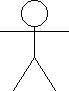
\includegraphics[width=0.4cm]{../img/stick.png}};

%% --------------- SERVING LAYER ------------------------------ %%
\node [component, right=of ghreads,xshift=20pt,yshift=-20pt] (servqh) {Query Router};
\node [multipledb, right=of servqh,xshift=-8pt,yshift=0cm] (servdb1) {Query Store 1};
\node [multipledb, below=of servdb1,xshift=0pt,yshift=20pt] (servdbn) {Query Store n}
	edge[dotted] (servdb1);
\node [above=of servqh,xshift=30pt,yshift=-15pt,ital] (servtitle) {Serving Layer};

	%% ----- phantom anchor node for db background border end point
\node [below=of servdbn,xshift=0pt,yshift=1cm+3pt] (servdbend) {};


%% --------------- BATCH LAYER ------------------------------ %%
\node [innercomponent, below=of gser,xshift=10pt,yshift=10pt] (bdeser) {Deserializer};
\node [component, below left=of bdeser,xshift=1cm+10pt,yshift=20pt] (bwriter) {Writer};

\node [component, below=of bwriter,yshift=0pt] (bformatter) {Formatter};
\node [database, right=of bformatter,yshift=-5pt] (bfile) {File System\\HDFS};
\node [innercomponent, right=of bfile,xshift=-1cm+20pt,yshift=30pt] 
							(bassembler) {Query Assembler};
%	

\node [component, below right=of bassembler,xshift=-2cm,yshift=20pt] (mapreduce) {Map-Reduce}
	edge[pre,bend right] node [elab,xshift=5pt] {run} (bassembler)
	edge[post] node [elabs] {read all records} (bfile)
	edge[post, bend right] node [elab,xshift=-25pt] {delete and rewrite} (servdbend);
\node [right=of bwriter,xshift=1cm,yshift=0pt, ital] (btitle) {Batch Layer};


\begin{pgfonlayer}{background}
	\node [subsys, 
			fit=(streamproc) (speeddb)]
		{};
\end{pgfonlayer}

\begin{pgfonlayer}{background}
	\node [subsys, black!10,
			fit=(gser) (ghwrites) (ghreads)]
		{};
\end{pgfonlayer}

\begin{pgfonlayer}{background}
	\node [subsys, blue!10,
			fit= (servtitle) (servqh) (servdb1) (servdbn)]
		{};
\end{pgfonlayer}

\begin{pgfonlayer}{background}
	\node [dotted,thick,draw,inner sep=4pt,
			fit=  (servdb1) (servdbn)]
		{};
\end{pgfonlayer}

\begin{pgfonlayer}{background}
	\node [subsys, yellow!30,
			fit=  (bwriter) (bdeser)  (bformatter) (bfile) (bassembler) (mapreduce)]
		{};
\end{pgfonlayer}
\end{tikzpicture}
\end{document}